\documentclass[a4paper,12pt]{article}
\usepackage{amsmath}
\usepackage{enumitem}
\usepackage{tikz}

\usetikzlibrary{arrows}

\begin{document}

\title{A local search approach for flexible job shop problems}
\author{Alex van Poppelen}
\date{\today}
\maketitle

\begin{abstract}

This is my abstract.

\end{abstract}

\tableofcontents

\section{Introduction}

\subsection{General introduction}

The Job Shop problem looks at the problem of scheduling multi operation jobs on a set of machines, where each operation in a job needs to be processed on a certain machine. The Job Shop problem is well known to be NP-hard in the strong sense, and notoriously difficult to solve even compred to other NP-hard problems.

In this paper, the Flexible Job Shop (FJS) and the Flexible Blocking Job Shop (FBJS) problems are considered. These two problems are an extension of the Job Shop and Blocking Job Shop problems where individual machines required by each operation are replaced by a number of identical machines running in parallel. Because of the need to assign operations to machines, the FJS is even more complex than the classical Job Shop problem. It is known to be strongly NP-hard \cite{approxfjsp}.

In the remainder of the first section, the FJS is formally defined. The blocking constraint is also explained. In the second section, a local search approach to solve the FJS is explored. Finally, the local search approach is modified to accomodate the blocking constraints in the third section.

\subsection{Formal definition}

The Flexible Job Shop problem is defined as follows.

\subsubsection{Notation}

We are given a set of $n$ jobs.

\[ \mathcal{J} = \{J_1, \dots, J_n\} \]

Each job $J_i$ consists of a fixed sequence of operations, where $o_i$ refers to the number of operations in the job:

\[ \mathcal{O}_i = \{O_{i,1}, \dots, O_{i, o_i}\} \]

Where $\mathcal{O}$ refers to the set of all operations. Each operation $O_{i,j}$ must be processed on a predetermined machine type.

\[ T_{i,j} \in \mathcal{T} = \{T_1, \dots, T_t\} \]

Each machine type $T_k$ has a given number of machines, defined as $m_k$. Furthermore, each operation $O_{i,j}$ has a processing time $p_{i,j}$ and a delay time $w_{i,j}$.

Machines are assumed to be continuously available from time 0, and can complete at most one operation at a time. Preemption is not allowed; the processing time $p_{i,j}$ must be uninterrupted. The delay time $w_{i,j}$ is defined as the time that must pass after operation $O_{i,j}$ is completed, before $O_{i,j + 1}$ may begin. Note that the machine $O_{i,j}$ was being processed on is immediately available.

\subsubsection{Objective}

We are interested in the following objective function.

\[ \min \{ C_\text{max} \} \]

Where $C_\text{max}$ is defined as the maximum completion time, or the time at which the last machine finished. This will be referred to as the \emph{makespan} of a schedule for the rest of this paper.

\subsubsection{Definition considerations}

In some other literature describing the Flexible Job Shop problem, there is no concept of a machine type. Instead, each operation is defined to be processed on some subset of the set of all machines \cite{approxfjsp}. This formulation is more general than the one used in this paper.

As a result, our definition of the FJS may exclude applications in settings that combine machines suited to highly specific tasks with more generalized machines, capable of processing a larger variety of operations.

\subsection{Blocking constraint extension}

In some situations, it may be unrealistic to model a scheduling problem as a Flexible Job Shop instance. For example, a manufacturing scenario might introduce storage space constraints. The FJS assumed that a job finished processing on one machine could be removed and placed into an intermediate buffer immediately, while waiting for it to be scheduled onto the next machine. This assumption may be unrealistic, and a factory might not have room for any intermediate buffers.

We can extend the problem definition to account for these constraints. In the Flexible Blocking Job Shop problem, a machine that is finished processing a job will be blocked until that job can be moved and processed by a successive machine. Note that this definition removes the distinction between the processing times and waiting times defined above, since the machine will be blocked for the duration of the waiting time regardless of whether subsequent machines are available or not.

\section{A local search approach to the FSJ}

In solving the FSJ, we are tasked with two problems. The first is to assign operations to machines. The second is to define an order on the set of operations assigned to every machine. We can choose to tackle these problems independently, or at the same time. In the independent approach, the operations would first be assigned to machines, reducing the problem to the classical Job Shop. In this paper, we will choose to tackle the problems at the same time, using a more complex schedule serialization function.

\subsection{Representation}

The classical Job Shop problem is often modeled as a disjunctive graph (for example, see \textbf{Figure 1}), where the directed arcs represent the precedence constraints within a job, and the undirected edges represent operations that must be processed on the same machine. By defining a direction on the edges, and making sure that these definitions result in an acyclic graph, one obtains a valid schedule for the Job Shop instance. In this case, an undirected edge represents a non-simultaneity constraint -- the two operations may be processed in any order, but not at the same time. If we wish to use the same definition for the FSJ, we are forced to assign operations to machines before directing the edges. However, that splits the problem into two parts as mentioned above, and will increase the complexity of the neighborhood. We will take another approach.

\begin{figure}
\centering
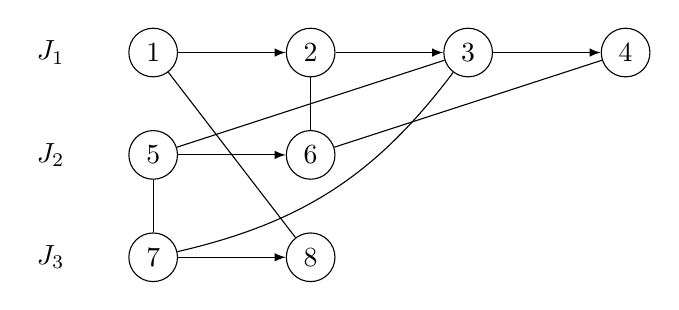
\begin{tikzpicture}

\tikzset{vertex/.style = {shape=circle,draw}}
\tikzset{arc/.style = {->,>=latex}}

% vertices
\node[vertex] (1) at  (0,0) {1};
\node[vertex] (2) at  (2,0) {2};
\node[vertex] (3) at  (4,0) {3};
\node[vertex] (4) at  (6,0) {4};
\node[vertex] (5) at  (0,-1.3) {5};
\node[vertex] (6) at  (2,-1.3) {6};
\node[vertex] (7) at  (0,-2.6) {7};
\node[vertex] (8) at  (2,-2.6) {8};

% labels
\node [left] at (-1,0) {$J_1$};
\node [left] at (-1,-1.3) {$J_2$};
\node [left] at (-1,-2.6) {$J_3$};

% arcs
\draw[arc] (1) to (2);
\draw[arc] (2) to (3);
\draw[arc] (3) to (4);
\draw[arc] (5) to (6);
\draw[arc] (7) to (8);

% edges
\draw (1) to (8);
\draw (3) to (5);
\draw [bend left=20] (3) to (7);
\draw (5) to (7);
\draw (2) to (6);
\draw (4) to (6);

\end{tikzpicture}
\caption{A disjunctive graph representing 3 jobs on 3 machines}
\end{figure}

We decide to modify the definition of an undirected edge. Instead, it will define two operations that may be processed in any order on the same machine, or independently on two different machines of the same type. Directing these edges will define the order of processing in the case the operations are on the same machine. In the case that they aren't, it only means that the start time of the second operation is equal to or greater than the start time of the first operation. This will make the serialization of a schedule more difficult, but the advantage is that generating the neighborhood will be easier.

In our representation, we can ascertain the following information from \textbf{Figure 1}. There are three jobs. Operations 1 and 8 must be processed by the same machine type. Similarly, operations 2, 4, and 6 are processed on another, and 3, 5, and 7 on the last machine type.

\subsection{Serializing the schedule}

Once all the edges in the disjunctive graph have been given directions, such that the graph is acyclic, it is possible to generate the schedule. The serialization function will assign operations to machines, and calculate the start time for each operation. The makespan can be determined after this process. It is important that the graph representation combined with the serialization function spans the entire set of feasible schedules. Furthermore, the serialization function should be deterministic in order to allow the local search to do its work.

To do this, we place the unscheduled operations in ordered queues for each machine type $T_k$. We take the first operation that has no unscheduled job predecessor, and schedule it greedily into the first available machine, taking care to schedule it at the same start time or after that of the previously scheduled operation for that type. This conforms to the requirements we laid out earlier in the representation section.

If there is no operation without an unscheduled job predecessor, then there exists a cycle in the graph, and the schedule serialization fails.

We could choose to apply tricks to generate a better schedule, but instead we will allow the local search to do that by modifying the order of the operations for each machine type.

\subsubsection{Schedule serialization example}

\begin{figure}
\centering
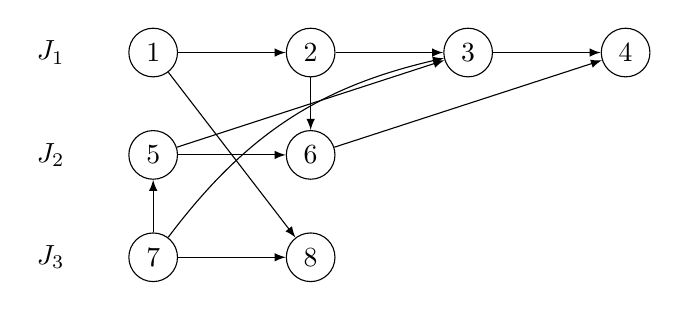
\begin{tikzpicture}

\tikzset{vertex/.style = {shape=circle,draw}}
\tikzset{arc/.style = {->,>=latex}}

% vertices
\node[vertex] (1) at  (0,0) {1};
\node[vertex] (2) at  (2,0) {2};
\node[vertex] (3) at  (4,0) {3};
\node[vertex] (4) at  (6,0) {4};
\node[vertex] (5) at  (0,-1.3) {5};
\node[vertex] (6) at  (2,-1.3) {6};
\node[vertex] (7) at  (0,-2.6) {7};
\node[vertex] (8) at  (2,-2.6) {8};

% labels
\node [left] at (-1,0) {$J_1$};
\node [left] at (-1,-1.3) {$J_2$};
\node [left] at (-1,-2.6) {$J_3$};

% arcs
\draw[arc] (1) to (2);
\draw[arc] (2) to (3);
\draw[arc] (3) to (4);
\draw[arc] (5) to (6);
\draw[arc] (7) to (8);

% edges
\draw[arc] (1) to (8);
\draw[arc] (5) to (3);
\draw[arc] [bend left=20] (7) to (3);
\draw[arc] (7) to (5);
\draw[arc] (2) to (6);
\draw[arc] (6) to (4);

\end{tikzpicture}
\caption{An acyclic directed graph representing a schedule}
\end{figure}

Consider the acyclic directed graph in \textbf{Figure 2}. The serialization function would set up three ordered queues.

\[ O_1 \rightarrow O_8 \]
\[ O_2 \rightarrow O_6 \rightarrow O_4 \]
\[ O_7 \rightarrow O_5 \rightarrow O_3 \]

Since operation $O_2$ has an unscheduled job predecessor, the algorithm would schedule $O_1$ or $O_7$ at time 0 on their respective machines first. After $O_1$ is scheduled, $O_2$ would become available to be scheduled at time $p_{1,1} + w_{1,1}$ or later. The algorithm continues until all the queues are empty or a cycle has been found. In the first case, the makespan is easily determined as the largest finish time for all the operations.

\subsection{Critical path neighborhood}

A neighborhood solution is generated by calculating the longest path 

\section{A local search approach to the FBSJ}

\begin{thebibliography}{9}

\bibitem{approxfjsp}
	Jansen, Klaus, Monaldo Mastrolilli, Roberto Solis-Oba.
	``Approximation algorithms for flexible job shop problems.''
	\textit{LATIN 2000: Theoretical Informatics}. Springer Berlin Heidelberg, 2000. 68-77.

\bibitem{genbjs}
	Heinz Gr{\"o}flin, Andreas Klinkert.
	``A new neighborhood and tabu search for the Blocking Job Shop.''
	\textit{Discrete Applied Mathematics}. 157 (2009): 3645-3655.

\bibitem{jobshopinfo}
	Beasley, J.E. 
	``Job shop scheduling''
	\textit{OR-Library}.
	Website, January 2016. http://people.brunel.ac.uk/~mastjjb/jeb/orlib/jobshopinfo.html.

\end{thebibliography}

\end{document}
